\section{Rosenbrock Function}
\label{sec:rosenbrock_function}
  The Rosenbrock function is a non-convex function used as a performance test 
  problem for optimization algorithms introduced by Howard H. Rosenbrock in 
  1960\footnote{
    Rosenbrock, H.H. (1960). \enquote{An automatic method for finding the
    greatest or least value of a function}. The Computer Journal. 3 (3): 
    175-184. doi:10.1093/comjnl/3.3.175. ISSN 0010-4620.
  }. 
  The global minimum is inside a long, narrow, parabolic shaped flat valley.
  To find the valley is trivial.
  To converge to the global minimum, however, is difficult.

  \begin{definition}[Rosenbrock function]
    The \emph{Rosenbrock function}, \(f: \mathbb{R}^n \rightarrow \mathbb{R}\), 
    is defined as:

    \begin{equation}
      \label{eq:rosenbrock_function}
      f(\mathbf{x}) 
        = \sum_{i=1}^{n-1} \left[ 
          100 (\mathbf{x}_{i+1} - \mathbf{x}_i^2)^2 + (1 - \mathbf{x}_i)^2 
        \right]
    \end{equation}

    where:

    \begin{itemize}
      \item \(n\) is the number of dimensions.
      \item \(\mathbf{x}\) is a vector of \(n\) real values.
    \end{itemize}
  \end{definition}

  The global minimum of the Rosenbrock function is \(f(\mathbf{x}^*) = 0\) at
  \(\mathbf{x}^* = (1, \ldots, 1)\).
  A contour plot and a surface plot of the Rosenbrock function for \(n = 2\) are
  shown in \vref{fig:rosenbrock_function}.

  \begin{figure}[ht!]
    \centering
    \begin{subfigure}[b]{0.4\textwidth}
      \centering
      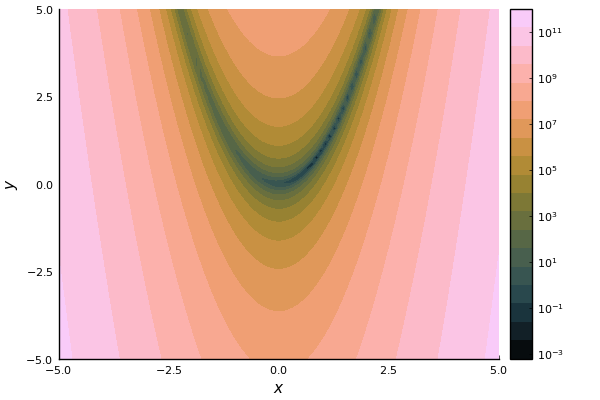
\includegraphics[width=\textwidth]{img/test_functions/rosenbrock_contour.png}
    \end{subfigure}
    \begin{subfigure}[b]{0.4\textwidth}
      \centering
      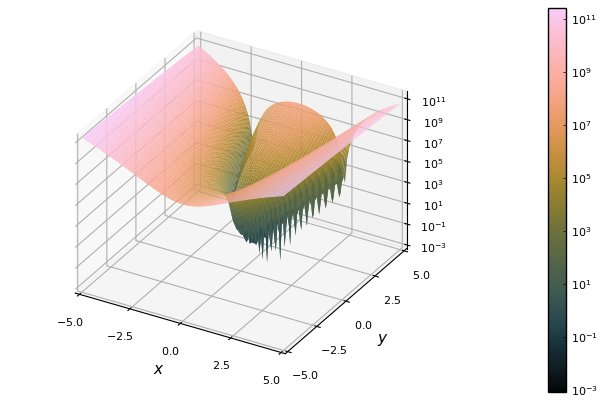
\includegraphics[width=\textwidth]{img/test_functions/rosenbrock_surface.png}
    \end{subfigure}
    \caption{Rosenbrock Function for \(n = 2\)}
    \label{fig:rosenbrock_function}
  \end{figure}